% Created 2018-05-09 Wed 13:08
\documentclass[9pt, b5paper]{article}
\usepackage{fontspec}
\usepackage{graphicx}
\usepackage{xcolor}
\usepackage{xeCJK}
\setCJKmainfont[BoldFont = Songti SC Bold, ItalicFont = STFangsong]{Songti SC}
\setCJKsansfont{STHeiti}
\setCJKmonofont{STFangsong}
\usepackage{multirow}
\usepackage{multicol}
\usepackage{float}
\usepackage{textcomp}
\usepackage{geometry}
\geometry{left=0.1cm,right=0.1cm,top=0.1cm,bottom=0.1cm}
\usepackage{algorithm}
\usepackage{algorithmic}
\usepackage{latexsym}
\usepackage{natbib}
\usepackage{listings}
\usepackage{minted}
\usepackage[xetex,colorlinks=true,CJKbookmarks=true,linkcolor=blue,urlcolor=blue,menucolor=blue]{hyperref}
\author{deepwaterooo}
\date{\today}
\title{AR First App}
\hypersetup{
  pdfkeywords={},
  pdfsubject={},
  pdfcreator={Emacs 25.3.1 (Org mode 8.2.7c)}}
\begin{document}

\maketitle
\tableofcontents


\section{Udpates}
\label{sec-1}
\begin{itemize}
\item All major functionalities are finished. One screen shot was attached. 

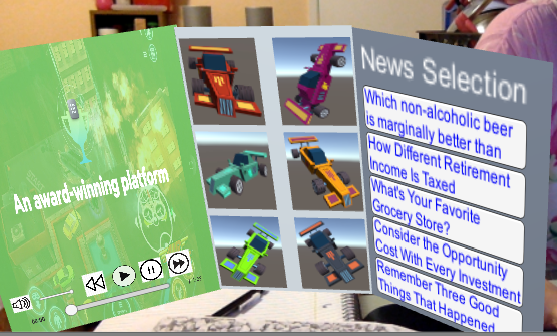
\includegraphics[width=.9\linewidth]{./pic/one.png}
\begin{itemize}
\item Will continueously smooth the project a little bit more (maybe a couple of days) to see if there is anything else that I can do for it.
\end{itemize}
\item video play part user interaction are completely finished. Will fill in the rest necessary components for news selection section to complete.
\item Play Pause function works, interface needs to be improved.
\item will make video user interaction work first, then modify others. 
\begin{itemize}
\item video works only without user interaction (play, pause)
\item car selection secton works
\item news selection basically works, hard coded five news, display in a new plain
\item Others: news API call works, NewsAPI client library works
\end{itemize}
\end{itemize}
% Emacs 25.3.1 (Org mode 8.2.7c)
\end{document}